%Bemerkung: Diese Datei wird über den \input{<name>.tex} in einer anderen .tex Datei %eingebunden. Daher müsst ihr euren Kram einfach nur noch runterschreiben
%Beispielsweise: 
\section{Software - Design}
\subsection{Usecases}
The flying software is definied by 12 different usecases and three actors. \\ \\
The Controller Actor represents the most complex actor system in this project. It uses the Analog Digital Converter (ADC) of the STM32F779 Controller and three external ADC to measure the temperature or the resistance of the strain gauge. \\ \\ 
The Usecase \textit{ADC external Request} describes the SPI communication to the three external ADCs. One ADC is used for two channels, there will be one strain-gauge per channel.  Therefore each channel are sampled with  one kSample per second. \\ \\
The second ADC usecase \textit{ADC Internal Request} is for sampling the temperature from a PT-100 sensor. Therefore its enugh to sample with 20 samples per second. \\ \\
\textit{Telemetry} covers each communication with the REXUS Serice Module. It includes the \textit{Error Handling} and \textit{Compression} usecase. Each time the microcontroller ($\mu C$) wants to send something to earth, this usecase is called. After each transmission, the REXUS Service Module will return the current error rate. So the telemetry has to adjust thier speed to maintain a soild communication. \\ \\
The \textit{Memory Usage} usecase describes how the memory is used. It is called each time the $\mu C$ saves something to flash memory. The controller have to save each measurment result and meta information about the flight, communication quality and in-flight problems. 
This usecase includes \textit{Write To Memory}, \textit{Read From Memory} and \textit{Reset Memory}. Each event will be triggered via \texit{USB} and \textit{DAPI}. The main reason why we did not connect these usecases is, that the mircocontroller has to act  first.  \\ \\ 
\textit{Debug}, this usecase describes the communication from Ground Station Software to the Controller. Therefore will be an JTAG interface implemented, connected via \textit{USB}. In pre-flight it will be used to gather information about the mechanical testcases. This is part of the  \textit{DAPI}\\
\textit{DAPI} for \textit{D}ata \textit{a}nd \textit{p}rogramming  \textit{i}nterface, describes the communication from ground station software to the microcontroller. 
\begin{figure}[htbp]
	\centering
	  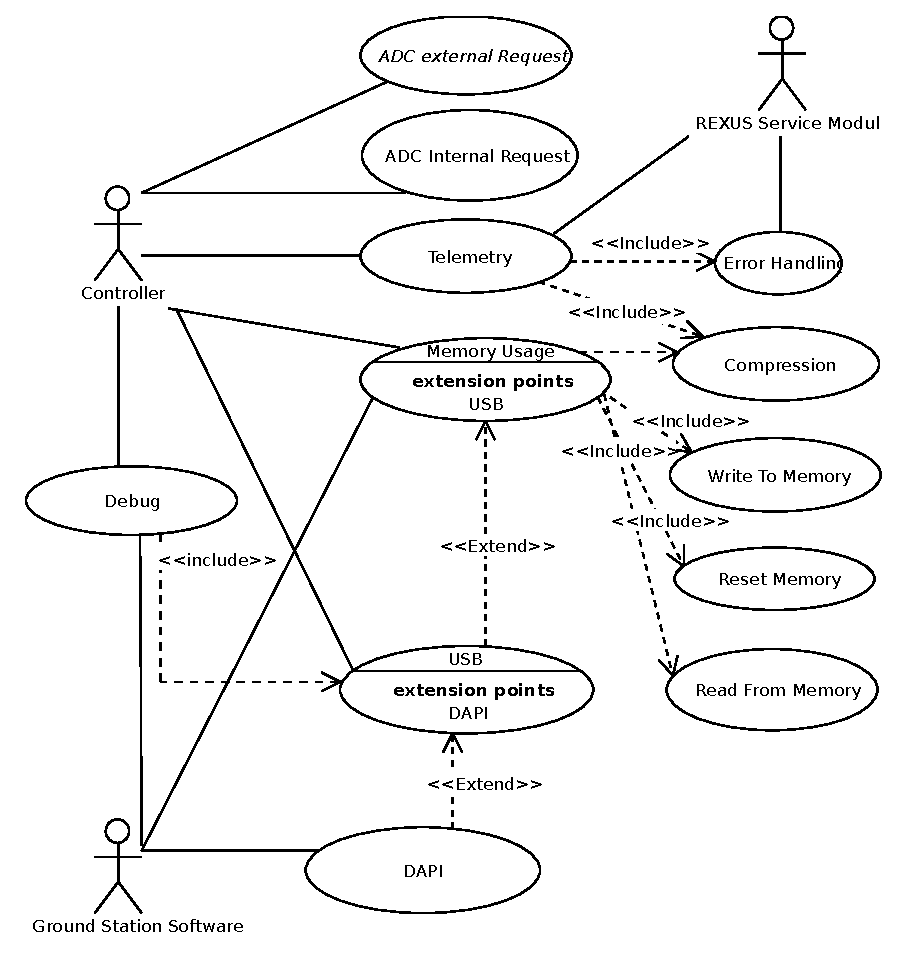
\includegraphics{HERMESS_USECASE.eps}
	\caption{EPS Image}
\end{figure}
\begin{figure}[htbp]
	\centering
	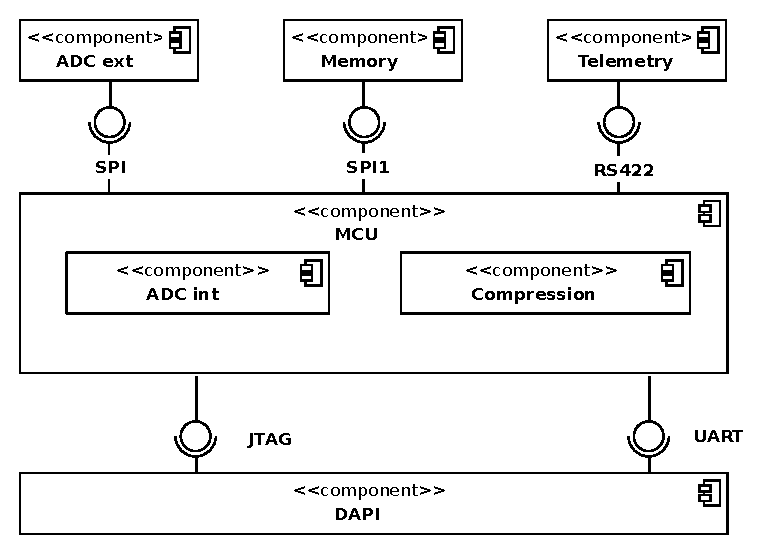
\includegraphics{Components.eps}
	\caption{SVG Image}
\end{figure}
